\documentclass[a4paper, 10pt]{article}
\usepackage{comment} % enables the use of multi-line comments (\ifx \fi) 
\usepackage{lipsum} %This package just generates Lorem Ipsum filler text. 
\usepackage{fullpage} % changes the margin
\usepackage{graphicx}
\usepackage{xcolor}
\usepackage[]{algorithm2e}
\usepackage{listings}

\begin{document}
%Header-Make sure you update this information!!!!
\noindent
\large\textbf{Middleware Project - MPI/OpenMP} \hfill \textbf{Marco Bacis} 873199 \\
Prof. Guinea \hfill \textbf{Daniele Cattaneo} 874757 \\
Prof. Mottola

\section*{Problem Statement}
The goal of the project is to develop a system to provide analytics over high velocity sensor data originating from a soccer game.
The goal of the analysis is to report and update the ball possession time for each player and team periodically during the game.
The data used comes from the DEBS2013 challenge, in which a number of wireless sensors embedded in the shoes and a ball were used during a soccer match, spanning the whole duration of the game
The main requirements is to use OpenMP and/or MPI to compute the real-time statistics.

\subsection*{Ball possession conditions}
A player is considered in possession of the ball when:
\begin{itemize}
\item He is the player closest to the ball
\item He is not farther than K meters from the ball
\item Ball possession is undefined whenever the game was paused
\end{itemize}

\subsection*{Additional Information}
\begin{itemize}
    \item The arm/shoe sensors send data at 200Hz, while the ball sensor has a rate of 2kHz
    \item As found from the DEBS2013 challenge paper, the field is half the dimension of a standard soccer field (66 x 52 meters)
    \item Each player (and even the referee) has 2 sensors, one for each shoe. The goalkeeper has 4 sensors (1 more for each hand)
    \item During the last 2.5 minutes before the first half ends, there are significant dropouts in the sensor data
    \item 4 balls are used during the game, but only the one inside the field is used for the possession computation
\end{itemize}

\section*{Implementation}

\subsection*{Serial Implementation}
In order to compute the ball possessions, the algorithm first divides the sensor data into a set of {\bf time-steps} based on the sensor's data rate.
%After that, for each timestep the nearest player can be found and its possession time updated.
In this case, given that the slowest sensor has a 200Hz rate, the timestep-based grouping of the records is done by dividing each record's timestamp (in picoseconds) by $1 / 200 = 0.005s = 5\,000\,000\,000ps$.
This is done while loading the game records file.

The ball sensor outputs data at 2kHz, so for each timestep group there are about 10 ball records for each ball (thus, 30 ball record in the first half and 40 in the second half). Conversely, the player sensors output data at 200Hz; thus in each time step there is one record for each player sensor.
To compute the ball possession, for each group and ball record we find the nearest player to the ball. The timestep of 5ms is distributed among these distinct positions of the ball.
The metric used to determine the nearest player to the ball is only the ground-based distance, as it was seen (by watching the match videos and pairing them to the ball's positions) that the $z$ coordinate reported by the sensors was too imprecise. 
Additionally, especially for small values of $K$, considering $z$ would also mean not considering some moves by the player as granting possession, while it would make sense to. For example, if a player hits the ball with their chest, since the chest is more than one meter above the feet, the ball would not be considered in possession by that player when $K=1$, even though the player is touching the ball.
The algorithm's pseudocode is shown in Algorithm~\ref{algorithm:main_loops}.

\begin{algorithm}[h]
    \SetKwInOut{Input}{input}
    \SetKwInOut{Output}{output}

    \Input{Full game sensor records $R$, set of game interruptions, $K$, $T$}
    \Output{Possession results for each interval of T seconds}
    \BlankLine
    \ForEach{game step $s \in R$}{
    	$bucket \longleftarrow (s.timestep - ($timestamp of the start of the game$)) / T$\;
      \If{game is not interrupted at time $s.timestep$}{
                $B \longleftarrow \emptyset$\tcc*[r]{set of ball records}
                $P \longleftarrow \emptyset$\tcc*[r]{set of player records}
                \tcp{Gather the records}
                \ForEach{record $r \in s$} {
                    \uIf{$r$ is a ball {\bf and} $r$ is inside the field}{
                        $B \longleftarrow B \cup r$\;
                    }
                    \uElseIf{$r$ is a player}{
                        $P \longleftarrow P \cup r$\;
                    }
                }
                \tcp{Compute the actual possession}
                $increment \longleftarrow 5ms / |B|$\;
                \ForEach{ball record $b \in B$}{
                    $minDist \longleftarrow INT\_MAX$\;
                    $minPlayer \longleftarrow \emptyset$\;
                    \ForEach{player record $p \in P$}{
                        $dist \longleftarrow \sqrt{(p.x-b.x)^2 + (p.y-b.y)^2}$ \tcc*[r]{ground distance}
                        \If{$dist < minDist$}{
                            $minDist \longleftarrow dist$\;
                            $minPlayer \longleftarrow p$\;
                        }
                    }
                    \If{$minDist < K$}{
                        $possession_{bucket}[minPlayer] \longleftarrow possession_{bucket}[minPlayer] + increment$
                    }
                }
       }
    }
    \caption{Main algorithm for ball possession computation}
    \label{algorithm:main_loops}
\end{algorithm}

\subsection*{Parallelization}

To parallelize the algorithm, we used OpenMP only, because the relatively small amount of data and the relative simplicity of the computation are such that using a network connection between computational nodes would add an amount of overhead comparable to the speedup.
In fact, a first look at the running time shows that the majority of the time is passed reading the csv file from disk.
%This means that, even if the algorithm can be parallelized, the running time will not be affected much, and the processing time is too low to gain much advantage by transferring the workload to other systems.

Given that the file reading is sequential, the parsing has been implemented in parallel to it, by using \emph{pipelining} between two parallel sections of code (reading $\rightarrow$ parsing). To achieve this we used the \texttt{omp sections} pragma.

The parallelized computation is split in two distinct loops. The first -- and most important -- loop is shown in Algorithm~\ref{algorithm:main_loops}. it computes -- for each time interval T, which we call \emph{bucket} -- the ball possession statistics for each player during that time interval only.
This loop does not perform an explicit enumeration of each time interval. The time interval in which each record belongs is computed from the timestamp independently.
We used the \texttt{omp parallel} pragma to let OpenMP parallelize the loop (which is possible because there are no inter-iteration dependencies). To protect the updating of the possession array from concurrency hazards, we used the \texttt{omp atomic} pragma. 
Compared to the algorithm shown above, the implementation collects some extra statistics regarding the number of records processed. Since these statistics are simple variable, we used the \texttt{omp reduction} pragma to ensure that they are correctly updated.

The second loop accumulates the data of each time step with the data of the previous steps, in order to compute the final cumulative statistics for the entire game. For example, after this loop has executed, the second bucket will contain the statistics for the entire first two $T$ periods of play instead of just the possession statistics of the second period $T$ of play.
This loop is less important to parallelize since the amount of data processed is several orders of magnitude lesser than in the main loop. Nevertheless, since each player's statistics are independent, we parallelized this computation "horizontally" using the \texttt{omp simd} pragma.

Finally, the accumulations are printed to screen (and can be redirected to a file).

\section*{Results}

The application has been tested on a Intel core i5-8259U CPU (2.30GHz, 4 cores, 8 threads) machine with 8GB of LPDDR3 DRAM.
In total, we performed 10 runs of 4 tests: K=1m,T=60s and K=5m,T=1s; serial (compiled without OpenMP) and parallel.

The results can be seen in Figure~\ref{fig:results}. The data reading part of the application hasn't gained much from the pipelining scheme, while the time of the computation time was considerably reduced (from 3.24 to 1.12 seconds for the K=1,T=60 case, and similar for the other).
The overall speedup is 1.24X, resulting from 1.20X for the file reading/parsing and 3.26X for the computation.
The computation speedup is very close to the number of physical cores, which indicates that parallelization has been effective (as the instruction mix of the threads is similar, hyperthreading is not useful).


\begin{figure}[h]
\centering
    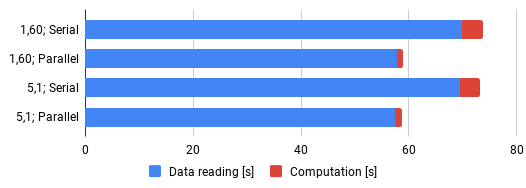
\includegraphics[width=0.5125\linewidth]{images/results.png}
    \caption{Performance tests results}
   \label{fig:results}
\end{figure}



\end{document}
